\documentclass[../main.tex]{subfiles}

\begin{document}

\section{Propriet\'a generali delle oscillazioni adiabatiche.}

\begin{todo}{Frequenza di \bv{}.}
qui o nella sottosezione precedente??
Kippenhan: 40.3, eigenspectra
Dalsgaard: notes 5.3Pg 83-
\end{todo}

\begin{comment}
\begin{figure}[!ht]
\centering
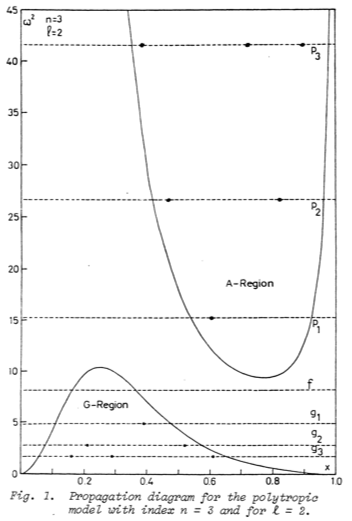
\includegraphics[width=\textwidth, height=0.9\textheight,keepaspectratio]{propagationAG}
\caption{Regioni di propagazione.}
\end{figure}
\end{comment}

\begin{todo}{dalsgaard 2005}
homology argument: scaling factor $\sqrt{GM}$
\end{todo}


\begin{todo}{Soluzioni numeriche e comportamentpo asintotico}
La soluzione numerica \'e dipendente dal modello di equilibrio: per il modello stellare $M4K$ viene riportata un precisione di $\SI{0.02}{\micro\hertz}$ (accuratezza \num{e-5}), mentre differenti valori della costante G fra quelli usati in letteratura risultano in differenze nelle frequenze calcolate di \numrange{-0.35}{-0.08}\si{\micro\hertz}, maggiori di quelle che risultano da differenti schemi di integrazione numerica.
\end{todo}

\begin{todo}{Numerical technique}
Inter-comparison of the g-, f- and p-modes calculated using different oscillation codes for a given stellar model

\end{todo}

\begin{todo}{Continous variation of parameter}
Problems in cowling vs full
\end{todo}

La soluzione numerica delle equazioni \eqref{eq:eigenomega}


\begin{comment}
\begin{figure}[!ht]
\centering
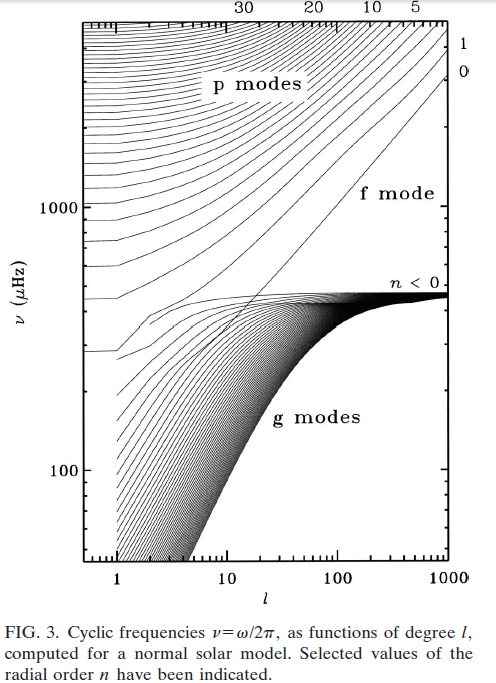
\includegraphics[width=\textwidth, height=0.9\textheight,keepaspectratio]{omega-l}
\caption{Modi di oscillazion. plot omega vs l..}
\end{figure}
\end{comment}

mostra due differenti comportamenti. Uso l'approssimazione asintotica per determinare la natura delle oscillazioni nelle due zone.

\clearpage

\subsection{Comportamento asintotico}


Per determinare la struttura dello spettro delle oscillazioni introduciamo l'approssimazione di Cowling (\cite{cow41oscillations}) cio\'e trascuriamo la perturbazione del potenziale gravitazionale. Quindi il sistema si riduce al secondo ordine

\begin{align}
&\frac{1}{r^2}\TDof{r}(r^2\xi_r)-\frac{\xi_rg}{c^2}+\frac{1}{\rho_0}(\frac{1}{c^2}-\frac{l(l+1)}{r^2\omega^2})P_1=0\label{eq:cowosc}\\
&\frac{1}{\rho_0}(\TDof{r}+\frac{g}{c^2})P_1-(\omega^2-N^2)\xi_r=0\nonumber
\end{align}

Considero i limiti asintotici di alte e basse frequenze: in entrambi ottengo un problema del tipo di Sturm-Liuville

\begin{todo}{Sturm-Liouville theory}
%https://en.wikipedia.org/wiki/Sturm%E2%80%93Liouville_theory
\end{todo}

\begin{todo}{Modi stabili/instabili}
Cox ??
\end{todo}

\begin{itemize}
\item Per $\omega\to\infty$:

Lo spettro \'e discreto con punto di accumulazione a $\omega=\infty$.
Le oscillazioni sono prodotte da onde acustiche in cui la forza dominante \'e fornita dalla pressione, chiamati modi p, ordinati in base al numero di zeri di $\xi_r$ fra il centro e la superficie. I modi p sono stabili.

\item Per $\omega\to0$:

Lo spettro \'e discreto con punto di accumulazione a $\omega=0$.
Il moto \'e determinato dalla forza di gravit\'a, chiamati modi g (ordinati secondo il numero di nodi radiali). La stabilit\'a dei modi g \'e detrminata dalla stabilit\'a convettiva: dato che $\omega^2_{Ad}=-grW$ il criterio di instabilit\'a convettiva si traduce in $rW>0$. Se $W<0$ in tutta la stella tutti i modi g sono stabili ($g_+$), se esistono zone in cui $W>0$ esistono anche modi g instabili ($g_-$).
\end{itemize}

Lo spettro solare \'e la combinazione dei modi parziali precedenti; il modo f separa  i modi g e p: non ha nodi in direzione radiale.

\subsection{Relazione di dispersione per i modi gravo-acustici.}

Approssimo il comportamento spaziale delle oscillazioni con quello di onda piana
\begin{align*}
&\vec{\xi}\propto\exp{i\scap{k}{x}},\ \vec{k}=k_r\hat{r}+\vec{k}_h\\
&S_l^2=\frac{l(l+1)c^2}{r^2}\approx k_h^2c^2
\end{align*}
e i coefficienti delle equazioni \ref{eq:cowosc} costanti ( approssimazione valida se la lunghezza d'onda delle perturbazioni \'e molto minore della scala caratteristica di variazione dei coefficienti).

\begin{todo}{Per poter parlare di onde}
Per poter parlare di onde devo assumere che la variazione di $P_0$ e $\rho_0$ abbiano lunghezze caratteristiche maggiori delle lunghezze di interesse (short-wave acustic):
\begin{align*}
&\PtwoDy{t}{\rho'}=-v_S^2\nabla^2\rho'\intertext{equazione d'onda per la propagazione della perturbazione}\\
&v_S=\sqrt{\frac{\Gamma_{1,0}P_0}{\rho_0}}&\intertext{adiabatic (Laplacian) sound speed.}
\end{align*}



Usando l'equazione di continuit\'a si vede che
\begin{align*}
&|\frac{\rho'}{\rho_0}|=\frac{v}{v_S}\\
&|\frac{\rho'}{\rho_0}|\ll1\ \Rightarrow \ \frac{v}{v_S}\ll1
\end{align*}
La teoria lineare \'e valida finch\'e la velocit\'a delle fluttuazioni associata alle onde acustiche \'e minore rispetto alla velocit\'a del suono.
Per l'equazione per la quantit\'a di moto linearizzata deve essere $\vec{c}\parallel \vec{k}$: la velocit\'a del fluido associato alle onde acustiche adiabatiche \'e parallela alla direzione di propagazione, pressure force supply the restoring force.

\end{todo}

Manipolando il sistema \ref{eq:cowosc} inserendo perturbazioni della forma (conservazione energia) $\xi_r\propto\rho_0\expy{-\frac{1}{2}}\exp{ik_rr}$, $P_1\propto\rho_0\expy{\frac{1}{2}}\exp{ik_rr}$:

\begin{align*}
&\frac{1}{r^2}\TDof{r}(r^2\xi_r)-\frac{\xi_rg}{c^2}+\frac{1}{\rho_0}(\frac{1}{c^2}-\frac{l(l+1)}{r^2\omega^2})P_1=0\\
&\frac{1}{\rho_0}(\TDof{r}+\frac{g}{c^2})P_1-(\omega^2-N^2)\xi_r=0\\
\\
&\xi_r=\frac{1}{(\omega^2-N^2)}[\frac{1}{\rho_0}(\TDof{r}+\frac{g}{c^2})]P_1\\
&\TDof{r}\xi_r=-\frac{2}{r}\xi_r+\frac{\xi_rg}{c^2}+\frac{1}{\rho_0}(\frac{1}{c^2}+\frac{l(l+1)}{r^2\omega^2})P_1\\
\\
&\TDof{r} \frac{1}{\rho_0}(\TDof{r}+\TDof{r} \frac{g}{c^2})P_1-(\omega^2-N^2)\TDof{r} \xi_r=0
\end{align*}

\begin{todo}{relazione dispersione stix pg 156 (5.33)}

Gough pg 792 eq 25-26

\end{todo}

Se considero $g$, $N$ e $c$ lentamente variabili rispetto alla lunghezza d'onda delle perturbazioni lo stesso vale per la lunghezza caratteristica della densit\'a $H=-\frac{\rho_0}{\TDy{r}{\rho_0}}=(\frac{g}{c^2}+\frac{N^2}{g})\expy{-1}$ e la frequenza di taglio acustica $\omega_A=\frac{c}{2H}$. Scrivo la relazione di dispersione

\begin{align}
&k_r^2=\frac{\omega^2-\omega_A^2}{c^2}+S_l\frac{N^2-\omega^2}{c^2\omega^2}\label{eq:localdispersion}\\
&=\frac{\omega^2}{c^2}(1-\frac{\omega_{l,+}^2}{\omega^2})(1-\frac{\omega_{l,-}^2}{\omega^2})\nonumber
\end{align}

\begin{comment}
\begin{figure}[!ht]
\centering
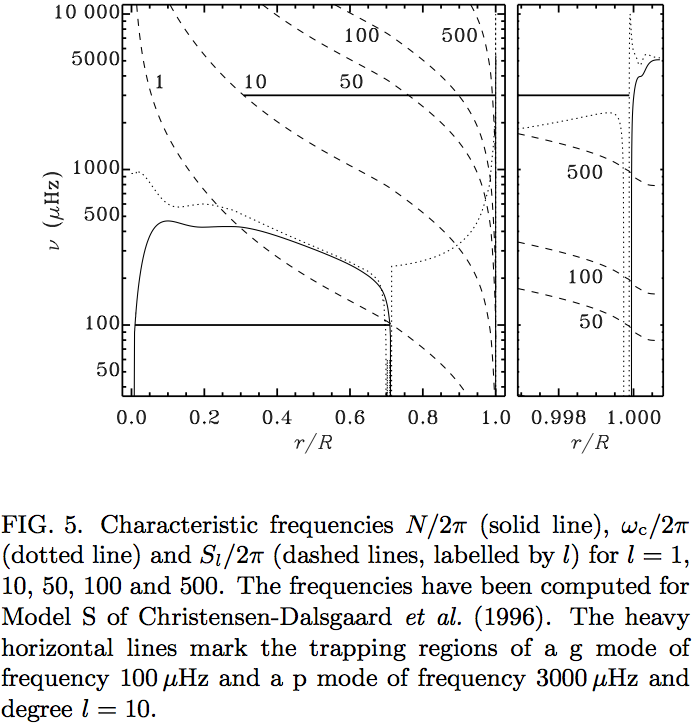
\includegraphics[width=\textwidth, height=0.9\textheight,keepaspectratio]{freqcaratt}
\caption{Frequenze caratteristiche.}
\label{fig:freqcaratt}
\end{figure}
\end{comment}

\clearpage


\section{Regioni di propagazione.}

\begin{comment}
\begin{figure}[!ht]
\centering
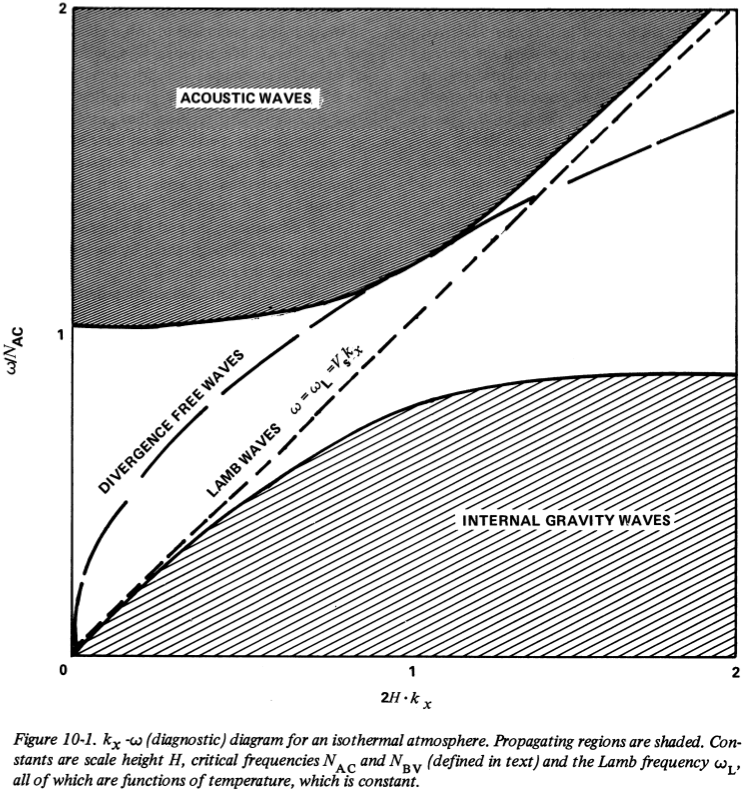
\includegraphics[width=\textwidth, height=0.8\textheight,keepaspectratio]{khomeagisot}
\caption{Diagramma frequenza numero d'onda orizzontale per atmosfera isoterma.}
\label{fig:khomeagisot}
\end{figure}

\begin{figure}[!ht]
\centering
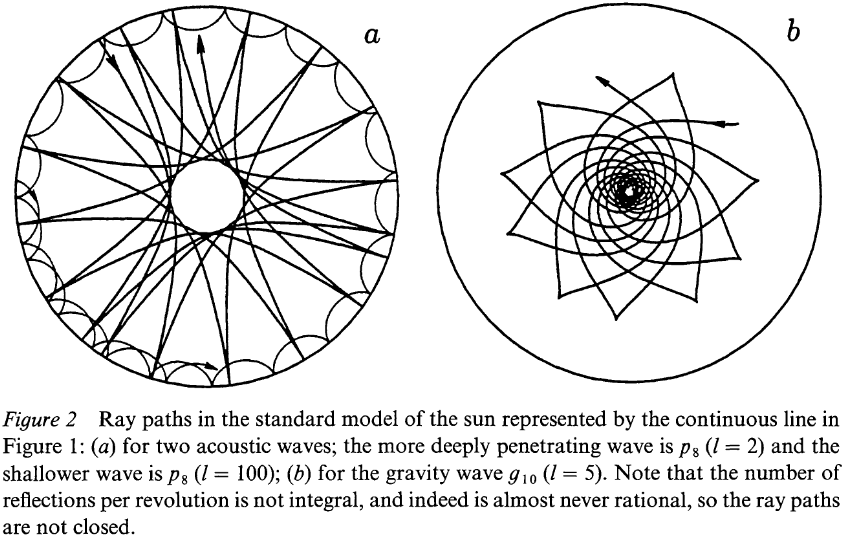
\includegraphics[width=0.9\textwidth, height=\textheight,keepaspectratio]{pgmodesC}
\caption{Cavit\'a risonanti per modi p e g.}
\label{fig:propagationAG}
\end{figure}
\end{comment}

Il comportamento oscillatorio richiede $k_r^2>0$.

I punti di inversione per le onde acustiche sono definiti da 
\begin{align*}
    &\omega^2=\frac{l(l+1)c}{r^2}&\intertext{large $k_hH$}\\
    &\omega=\omega_A&\intertext{small $k_hH$}
\end{align*}

per i modi g da
\begin{align*}
    &\omega=N&\intertext{large $k_hH$.}
    &\omega=(\frac{\omega_A}{N})ck_h&\intertext{small $K_hH$.}
\end{align*}

\'E possibile analizzare tramite metodo  JWKB il sistema di equazioni delle oscillazioni del secondo ordine in approssimazione di Cowling, previa oppurtuna trasformazione, da cui si ottiene la relazione valida per i modi
\begin{equation}\label{eq:jwkb}
\omega\int_{r_1}^{r_2}[1-\frac{\omega_A^2}{\omega^2}-\frac{S_l^2}{\omega^2}(1-\frac{N^2}{\omega^2})]\expy{\frac{1}{2}}\frac{dr}{c}\approx\pi(n-\frac{1}{2})
\end{equation}
dove $r_1$ e $r_2$ sono due zeri consecutivi del numero d'onda radiale e l'integrazione \'e in una regione di propagazione. Nel caso dei modi p e assumendo $S_l\ll\omega$ vicino al punto di inversione superiore ho

\begin{equation}\label{eq:jwkbmodep}
\omega\int_{r_1}^{r_2}[1-\frac{S_l^2}{\omega^2}]\expy{\frac{1}{2}}\frac{dr}{c}\approx\pi(n-\alpha{\omega})
\end{equation}

\clearpage

\subsection{Cavit\'a acustiche.}
Per grandi $\omega$ ~\ref{eq:localdispersion} si riduce alla relazione di dispersione acustica 

\begin{equation*}
\omega^2=c^2(k_r^2+k_h^2)
\end{equation*}


Posso ricavare il raggio di inversione del moto in direzione radiale $k_r=0$ dalla relazione di dispersione per onde onde acustiche, da cui segue
\begin{equation}
\frac{c(r_i)}{r_i}=\frac{\omega}{l(l+1)}
\end{equation}

Maggiore \'e il grado l (piccolo $\lambda_h$) meno profonda \'e la cavit\'a: sono riflesse verso la superfice quando la velocit\'a del suono \'e aumentata fino alla loro velocit\'a di fase orizzontale; la profondit\'a della cavit\'a acustica varia con il variare della scala orizzontale dell'onda. (Top  convection zone down to the level at which refraction due to sound speed increasing $c\propto\sqrt{T}$ turn the wave around when $c=\frac{\omega}{k_h}$)

Stima profondit\'a cavit\'a acustica
\begin{align*}
    &T=\Dcvar{\TDy{z}{T}}{Ad}\delta&\intu{$\delta$ \'e la profondit\'a sotto la fotosfera}\\
    &T=\Dcvar{\TDy{z}{T}}{Ad}=\frac{T}{P}\TDly{P}{T}|_{Ad}\TDy{z}{P}=\frac{\gamma-1}{\gamma R}g=\frac{g}{c_P}\\
    &c^2=(\gamma-1)g\delta&\intertext{da $c=\frac{\omega}{k_h}$ segue:}\\
    &\delta=\frac{\omega^2}{k_h^2(\gamma-1)g}
\end{align*}
minore la lunghezza d'onda orizzontale pi\'u sottile la cavit\'a.

Vicino alla superficie l'efficienza della convezione diminuisce, il gradiente di temperatura diventa fortemente sopra-adiabatico e la fraquenza critica $\omega_A$ aumenta notevolmente: le onde acustiche con periodo attorno ai 5-min diventano evanescenti in poche scale di altezza: l'inizio della zona convettiva \'e uno specchio a larga banda per onde acustiche. 

Duvall82

In un grafico $\frac{\omega}{k_h}$ vs $\frac{\pi(n+\alpha)}{\omega}$ i modi p sono rappresentati da un'unica curva. Se considero la differenza di fase
\begin{align}\label{eq:duvall}
&\Delta\phi=\int_{r_t}^{\rsun{}}k_r\,dr=\int_{r_t}^{\rsun{}}(\frac{1}{c^2}-\frac{l(l+1)}{r^2\omega^2})\expy{\frac{1}{2}}\,dr\\
&=F(\frac{\omega}{L})\\
&\Delta\phi=\pi(n+\alpha)
\end{align}
tra i bordi interno ed esterno della cavit\'a acustica per un modo di oscillazione $\Delta\phi=\pi(n+\alpha)$ la costante $\alpha$ \'e necessaria dato che i bordi non sono rigidi.
L'integrale risulta funzione di $\frac{\omega}{k_h}$. 

\begin{comment}
\begin{figure}[!ht]
\centering
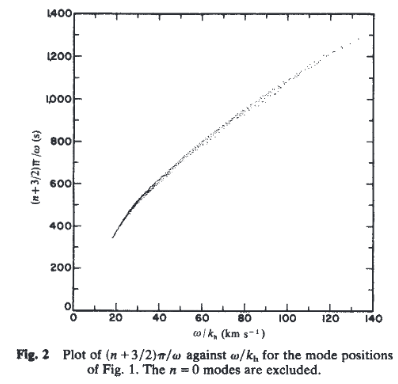
\includegraphics[width=\textwidth, height=0.9\textheight,keepaspectratio]{Duvall}
\caption{Legge di Duvall.}
\end{figure}
\end{comment}

\clearpage

\subsection{Cavit\'a risonanti per modi g.}

Nella parte a basse frequenze dei modi g la relazione \ref{eq:localdispersion} si approssima, per $l\neq0$ con

\begin{equation*}
k_r^2=\frac{S_l^2}{c^2}(\frac{N^2}{\omega^2}-1)
\end{equation*}

La regione dei modi g ha come limite superiore N per grandi l, la linea $\omega=\frac{S_lN}{\omega_A}$.

Per i modi g le regioni di propagazione sono quelle per la frequenza \'e minore di entrambi $N$ e $ck_h$.

La struttura degli strati esterni del sole \'e dominata dalla ionizzazione di H e He con conseguente aumento dell'opacit\'a e quindi del gradiente di temperatura in equilibrio radiativo e il calore specifico: il gradiente di temperatura critico per instabilit\'a convettiva $\frac{g}{c_P}$ diminuisce. In questa regione il gradiente di temperatura \'e debolmente super-adiabatico, $N^2<0$: la zona convettiva costituisce una barriera per le onde di gravit\'a interne.

Le onde di gravit\'a sono presenti nelle regioni in cui il gas \'e neutro o completamente ionizzato ($N^2$ grande) e sono riflesse in regioni dove $N$ \'e piccolo o immaginario: ionizzazione parziale, instabilit\'a convettiva, centro del Sole.

Ho cavit\'a risonanti per modi g:
\begin{itemize}
    \item Core radiativo.
    
    Tra la la parte centrale dove $g\to0$ e il fondo della zona convettiva dove $N^2<0$.
    \item Atmosfera.
    
    $N$ ha un massimo in coincidenza del punto $T_m$ nella cromosfera: modi g confinati tra zona convettiva e cromosfera ($\Pi\approx\numrange{180}{800}\si{\second}$).
\end{itemize}


\section{Analisi asintotica}

\begin{todo}{Analisi asintotica}
Vedi stix 5.3??

Heliosismic inference: observed vs predicted frequencies (Simple models and analytic (asyntotic) formula).
\end{todo}

\subsection{JWKB analysis}

\begin{todo}{cos'\'e l'analisi asintotica}
Vedi articolo gough07
\end{todo}

Nell'analisi tramite JWKB si tiene conto del fatto che le oscillazioni non sono puramente acustiche e le propriet\'a del gas non sono omogenee.

I modi osservati sono di alto ordine radiale o grado angolare: uso l'approssimazione di Cowling (ignoro la perturbazione al potenziale gravitazionale $\Phi'$).

\begin{align*}
&\omega\int_{r_1}^{r_2}\sqrt{1-\frac{\omega_c^2}{\omega^2}-\frac{S_l^2}{\omega^2}(1-\frac{N^2}{\omega^2})}\,\frac{dr}{c}\approx\pi(n-\frac{1}{2})\\
&\omega_c=\frac{c^2}{4H^2}(1-2\TDy{r}{H})\\
&H=-(\TDy{r}{\ln{\rho}})\expy{-1}
\end{align*}

\subsection{Asymptotic properties of p modes}

Posso trascurare N e, eccetto vicino alla superficie, $\omega_c\ll\omega$, mentr vicino alla superficie $S_l\ll\omega$ for small/moderate l.

\begin{align*}
&\omega\int_{r_1}^{r_2}\sqrt{1-\frac{\omega_c^2}{\omega^2}-\frac{S_l^2}{\omega^2}}\,\frac{dr}{c}\approx\pi(n-\frac{1}{2})&\intertext{where $r_1=r_t$, $r_2=R_t$. With help of our assumption we can expand the integral and, introducing the function $\alpha(\omega)$ depending only on frequency and near surface behaviour of $\omega_c$.}
\end{align*}

For low degree modes we use the fact that integrand differs from 1 only close to lower turning point close to center for low order mode ($F(w)\approx\int_0^R\frac{dr}{c}-w\expy{-1}\frac{\pi}{2}$)

\begin{align*}
&\nu_{nl}=\frac{\omega_{nl}}{2\pi}\approx(n+\frac{l}{2}+\frac{1}{4}+\alpha)\Delta\nu\\
&\Delta\nu=[2\int_0^R\frac{dr}{c}]\expy{-1}&\intu{is the inverse of twice travel time center/surface. This equation predict uniform spacing in n of frequency of low degree modes (claverie79)}
\end{align*}

Deviazioni da questa legge hanno potenziale diagnostico per la parte interna, infatti estendendo l'espansione di

\begin{equation*}
F(w)=\int_{r_t}^R\sqrt{1-\frac{c^2}{w^2r^2}}\,\frac{dr}{c}
\end{equation*}

fino al termine dipendente dalla variazione di c:

\begin{align*}
d_{nl}=\nu_{nl}-\nu_{n-1,l+2}\approx-(4l+6)\frac{\Delta\nu}{4\pi^2\nu_{nl}}\int_0^R\TDy{r}{c}\,\frac{dr}{c}&\intertext{sound speed is reduced as $\mu$ increases with H to He conversion as star ages: as a result $d_{nl}$ is reduced providing measure of evolutionary state of stars}
\end{align*}

\subsection{Asymptotic g modes}

In inner domain an expansion in terms of $\frac{\omega^2}{S_l^2}$ is possible, while $\frac{\omega^2}{N^2}$ serves as small expansion parameter in outer domain containing the surface, additional domains have to be considered for zeros of $N^2$

For the Sun we have $N^2(r_v)=0$ where $r_v$ marks lower bound of convection zone, matching the respective expansion we have in first order
\begin{align*}
&T_{n,l}=\frac{2\pi^2(n+\frac{l}{2}-\frac{1}{4})}{\sqrt{l(l+1)}}(\int_0^{r_v}\frac{N}{r}\,dr)\expy{-1}=\frac{n+\frac{l}{2}-\frac{1}{4}}{\sqrt{l(l+1)}}T_0
\end{align*}

g modes have equidistant period spacing.


\section{Excitation and damping. Ampiezza delle autofunzioni meccanismi di eccitazione delle oscillazioni solari.}

\subsection{$\kappa$ mechanism}

Suppose in phase of comperession opacity increases: the compressed layer then absorbs energy out of radiative flux toward stellar surface and thus will be heated in excess than mere adiabatic heating.

The subsequent compression will be stronger than preciding one.

\cite{zhe63variable} demonstrated that this mechanism of overstability drives the pulsation of $\delta$ cephei and related variable stars where is particularly effective in layer of He second ionization.

The crucial parameter measuring the opacity variation is 
\begin{equation*}
\kappa_T=\Dcvar{\PDly{T}{\kappa}}{P}
\end{equation*}

It has a maximum in the layer of partial H ionization: in this layer there is a strong driving but we must include contributions from all layers in order to see if a particular mode is excited or damping.

We must abandon adiabatic assumption and use actual energy equation: 
\begin{equation*}
c_P\rho(\PDy{t}{T}-\nad{}\frac{T}{P}\TDy{t}{P})=-\nabla\cdot\vec{F}
\end{equation*}
from \cite{and75nonadiabatic}: the second term on the left describes adiabatic heating/cooling and $\vec{F}$ is the energy flux.

Il sistema di equazioni che descrive le oscillazioni non e pi\'u autoaggiunto e le frequenze sono complesse.

\'e difficile determinare se un modo sia instabile o meno perch\'e \'e necessario tenere conto dello smorzamento causato dalle perdite radiative nell'atmosfera otticamente sottile e dell'interazione con i moti convettivi non stazionari: difficile da stimare.

Since relative growth rate are small, with $Q=\frac{\Re{\omega}}{\Im{\omega}}\approx10^3$ or larger for solar p modes there is not much certainty about sign of $\Im{\omega}$.

\subsubsection{Argument against excitation of solar p modes by means of $\kappa$ mechanism}

The excited/damped oscillator is represented by
\begin{equation*}
\ddot{\xi}-2\beta\dot{\xi}+\omega^2\xi=0
\end{equation*}

The net effects of all excitation and dumping yield the coefficient $\beta$: if excitation wins over damping $\beta>0$, then there is unlimited growth of this mode (the equation above is homogeneous and linear). It's only be means of non-linear terms neglected above and in oscillation equations that the growth could be held.

Before non-linear terms take effect the amplitud should be sizable unlike small amplitudes observed on the Sun.

\subsection{Stochastic excitation by convection}

L'interazione con la convezione e causa di smorzamento: un blob di gas che si muove avanti e indietro nel suo moto convettivo produce attrito come gli atomi agitati da moto termico e collisioni.

D'altra parte il gas racchiuso tra due pareti riflettenti \'e continuamente colpito/perturbato da blob di gas convettivi: analogo di una campana suona in maniera casuale a una trumphet excited with random spectrum and random phase jump.

Formalmente si descrive l'oscillatore con
\begin{equation*}
\ddot{\xi}-2\beta\dot{\xi}+\omega^2\xi=f(t)
\end{equation*}
dove $f(t)$ \'e una forzante stocastica.

The spectrum and amplitudes of excited modes is determined by forcing function.

Observed frequencies are in the range \SIrange{2}{5}{\milli\hertz}: the upper bound comes about because up to $l\approx2000$ ($2Hk_h\approx1$) the atmospheric acustic cutoff is at about \SI{5}{\milli\hertz} almost indipendent of horizontal wavenumber; at larger frequencies there is no total reflection and no eigenoscillations with discrete spectrum. For lower bound at about \SI{2}{\milli\hertz}: for high l there are no p modes at smaller frequencies, we see the smallest radial order including fundamental; at low l the oscillations of low frequencies have upper reflection boundariy so deep below photosphere that at observable layers the amplitude is undetectable with present technique.


\subsection{Wave propagation in atmosphere}

There is no acustic cutoff for frequencies higher than atmospheric value of $\omega_A$: instead of discrete eigenvalue we expect a continuum of propagating acustic waves clearly seen for frequencies above $\approx\SI{5}{\milli\hertz}$. The phase difference between two levels in atmosphere separated by $\Delta r$ is $\Delta\phi=k_r\Delta r$ and icreases with frequencies because $k_r\approx\frac{\omega}{c_s}$ at this high freq.

There is some phase propagation for frequencies below \SI{5}{\milli\hertz} within spectral band where discrete modes exist: the closer the frequency is to atmospheric $\omega_A$ the less perfect is the reflection of eigenmodes.

Staiger's diagram also indicates presence of IGW in solar atmosphere. The signature is the negative phase difference at low frequencies: using dispersion relation for isothermal atmosphere
\begin{equation*}
\frac{k_h^2(\omega^2-N^2)}{\omega^2(\omega^2-\omega_A^2)}+\frac{k_r^2}{\omega^2-\omega_A^2}=\frac{1}{c^2}
\end{equation*}
which for constant $\omega$ is a quadratic surface in $\vec{k}$ space.

The vector of phase propagation $\vec{k}$ is the radius vector, the group velocity, gradient $\PDy{\vec{k}}{\omega}$ is perpendicular to surface $\omega^2$ const.

In the region of propagating acustic wave the surfaces are oblate ellipsoid of revolution with respect to $k_r$ axis because $\omega^2>\omega_A^2$ (and $\omega^2>N^2$): in this case the vertical components of phase velocity and group velocity have the same sign.

A wave having its excitation deep in the atmosphere will propagate its energy upward and if it's of acustic nature will also propagate phase upward.

By contrast the obove dispersion relation will represent one-shell hyperboloid of revolution for IGW where $\omega^2<N^2$ (and $\omega^2<\omega_A^2$): the r component of phase and group velocity have different sign. An IGW excited from below with upward propagating energy will exhibits downward propagating phase (Vedi steigert intorno a \SI{1}{\milli\hertz}).

(IGW possible only for $N^2>0$ are in stably stratified layers the natural substitutes of convection which depends on $N^2<0$)

\subsection{$\epsilon$ mechanism}

The $\epsilon$ mechanism consist in amplified energy production in the phase of maximum compression (diesel engine): the mechanism would operate in region of max He3 accumulation and lead to growing perturbation because of strong T sensitive of \mblock{^3He(^3He,2p)\alpha} reaction of PPI chain. The g modes, having peak amplitude in deep core would most likely be excited.

Instability of g modes producing finite amplitude perturbation would destroy $^3He$ peak: intermittent manner with timescale approx \SI{e8}{\year}.

\stopcontents[chapters]

\end{document}